\chapter{Lezione 12 - Cloud computing}

Benvenuti a questa nuova lezione.
Parleremo di cloud computing.
Gli argomenti che tratteremo in questa lezione sono una definizione di riferimento e un insieme, commenteremo anche un insieme di definizione di cloud computing e presenteremo il modello di calcolo.

Argomenti trattati:

\FloatBarrier
\begin{figure}[H]
  \centering
  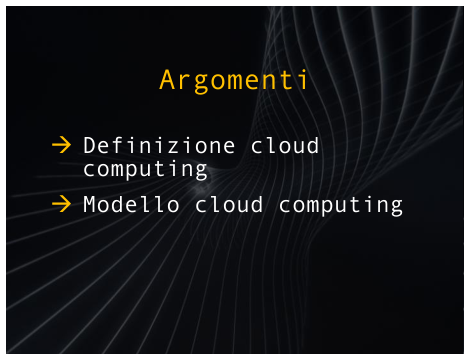
\includegraphics[width=0.50\textwidth,
                    trim=40 100 40 60, % L B R T
                    clip]
                    {images/Lez12_p01_fig_02}
  % \caption{Sommario}
  % \label{fig:Lez15_p06_fig_02}
\end{figure}
\FloatBarrier
\noindent

\section{Cloud computing} %00:31

Ma vediamo subito la definizione di cloud computing.

\FloatBarrier
\begin{figure}[H]
  \centering
  
\includegraphics[width=0.50\textwidth,
                    trim=100 120 100 80, % L B R T
                    clip]
                    {images/Lez12_p01_fig_04}
  % \caption{Sommario}
  % \label{fig:Lez15_p06_fig_02}
\end{figure}
\FloatBarrier
\noindent

Il National Institute of Standards and Technologies (NIST) è un laboratorio di definizione di misurazioni standard, quindi non un'agenzia di certificazione del governo americano.
È stata istituita nel 1901 e dal 1901 e all'1988 si chiamava National Bureau of Standards.

\FloatBarrier
\begin{figure}[H]
  \centering
  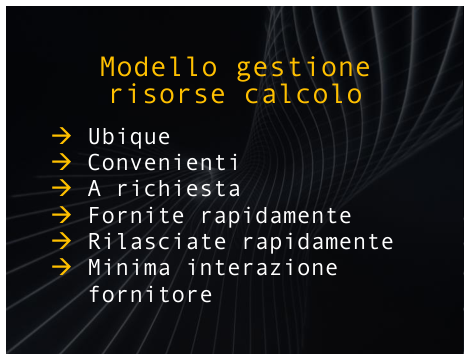
\includegraphics[width=0.50\textwidth,
                    trim=40 40 40 40, % L B R T
                    clip]
                    {images/Lez12_p01_fig_05}
  % \caption{Sommario}
  % \label{fig:Lez15_p06_fig_02}
\end{figure}
\FloatBarrier
\noindent

La prima definizione di cloud computing è stata presentata proprio da loro come modello per la gestione di risorse di calcolo ubique, cioè localizzate in qualunque posizione.

Non è rilevante dove la risorsa fisica è utilizzata per il calcolo, per la memorizzazione, qualunque tipo di risorsa venga utilizzata in questo modello cloud, non ha come riferimento rilevante la sua localizzazione fisica.

Inoltre possono essere considerati in questo modello di calcolo tutti i device periferici, cellulari, mobili che permettano un'interazione in qualunque posizione geografica dell'utente.

La gestione delle risorse con questo modello è conveniente; è possibile un risparmio economico perché non è necessario acquistare e gestire risorse fisiche ma solo per l'ammontare delle risorse che vengono effettivamente utilizzate per le computazioni o per i servizi che vengono richiesti.

La definizione prevede che l'utilizzo di queste risorse, e questa è una caratteristica fondante del modello, siano a richiesta.

A richiesta vuol dire che da una parte l'utente richiedente di un servizio cloud può fissare una soglia, un'ammontare di risorse da utilizzare, la potenza di calcolo piuttosto che la quantità di memoria di archiviazione, piuttosto che la larghezza di banda, ma le risorse sono anche poi valutate sulla base della necessità durante l'esecuzione delle computazioni e durante l'erogazione dei servizi.

Quindi se un programma, se una computazione sta arrivando alla fine dell'utilizzo e della memoria, ecco che il meccanismo di gestione del modello cloud fornisce memoria supplementare fino al completamento dell'esecuzione del programma.

Le risorse devono essere fornite rapidamente, quindi il meccanismo di gestione delle risorse, da una parte di misurazione, dall'altra di allocazione e fornitura delle risorse deve essere molto efficiente, perché i tempi di calcolo del servizio primario richiesto all'utente non devono essere eccessivamente appesantiti da questo sovraccarico gestionale.

Le risorse devono poter essere rilasciate rapidamente, alla fine dell'uso da parte di un'applicazione di una specifica risorsa, questa risorsa deve risultare già disponibile per un altro programma o un utente umano che ne facesse richiesta.

L'interazione del richiedente di un servizio con il sistema cloud o col fornitore del servizio deve essere minimizzata.

Il servizio deve poter richiedere l'erogazione e definire l'ammontare delle risorse di calcolo necessarie, quindi in qualche modo configurare il suo ambito di calcolo e interagire per la gestione amministrativa che gli è permessa, null'altro.

\FloatBarrier
\begin{figure}[H]
  \centering
  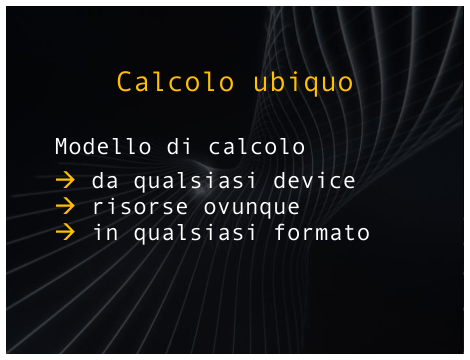
\includegraphics[width=0.50\textwidth,
                    trim=40 100 40 40, % L B R T
                    clip]
                    {images/Lez12_p01_fig_06}
  % \caption{Sommario}
  % \label{fig:Lez15_p06_fig_02}
\end{figure}
\FloatBarrier
\noindent

Vediamo nel dettaglio il significato di calcolo ubiquo: è un modello di calcolo che può essere eseguito o richiesto da qualsiasi device.

L'ubiquità del calcolo si riferisce sia alla indipendenza, al fatto che la localizzazione delle risorse che effettuano il calcolo sia trascurabile in questo modello, sia anche che l'utente che utilizza un device client per richiedere un servizio o i device stessi che possono gestire la computazione o richiedere automaticamente delle operazioni, possono essere localizzate in qualunque posizione geografica.

Le risorse di calcolo possono essere localizzate ovunque, possono essere organizzate in rete, in cluster di calcolatori, in cluster di memorie o essere gestite in maniera più autonoma, più indipendente, essere connessi in rete locale, in rete geografica o essere anche appartenenti o gestite da cloud, quindi sistemi di organizzazione in qualche modo autonomi o con un minimo di interazione per l'interoperabilità.

L'interoperabilità naturalmente è un fattore molto importante e il terzo elemento per il calcolo ubiquo è il formato, in qualsiasi formato.

Con qualsiasi formato indichiamo che sia i dati devono poter essere gestiti in qualsiasi formato, sia le richieste, quindi i protocolli di trasmissione gestiti, devono coprire la più ampia varietà possibile per fornire una maggiore elasticità, una maggiore estensione alle possibilità di tipo di calcolo, di servizio che possano essere erogate conformemente a questo modello.

\section{Strumenti di supporto} %08:20

\FloatBarrier
\begin{figure}[H]
  \centering
  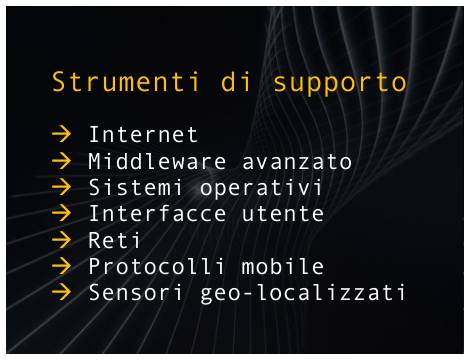
\includegraphics[width=0.50\textwidth,
                    trim=40 20 40 40, % L B R T
                    clip]
                    {images/Lez12_p02_fig_01}
  % \caption{Sommario}
  % \label{fig:Lez15_p06_fig_02}
\end{figure}
\FloatBarrier
\noindent

Gli strumenti di supporto per il calcolo ubiquo sono internet come infrastruttura di connessione, infrastruttura di rete che è diventato indubbiamente uno standard sia come infrastruttura fisica sia in quanto a servizi di supporto e protocolli che normano il funzionamento di questi servizi.

Il middleware avanzato è il sistema, la parte di gestione automatica di queste risorse per il loro accesso, per la loro richiesta e per la loro gestione, la locazione, assegnazione e rilascio.

Per quanto riguarda i sistemi operativi non abbiamo fatto riferimento nemmeno al tipo di macchine, al tipo di risorse fisiche che possono essere coinvolte, questo significa che in una nuvola, in un modello cloud, le risorse oltre a essere localizzate dove si voglia possono essere anche macchine di qualsiasi tipo, non sono posti vincoli o specifiche per le risorse che possano essere coinvolte, che possano contribuire alla realizzazione di questo modello, a maggior ragione i sistemi operativi.

Le interfacce utente devono essere agili ma devono essere anche facilmente conformabili, facilmente riconosciute dal sistema di base.

I servizi cloud sono attualmente e frequentemente gestiti da device mobili che hanno quindi una grandissima varietà sia tecnologica sia anche dovuta alla settorializzazione commerciale.

Le reti servono sia come connessione tra le varie risorse, sia per l'accesso alle risorse che devono essere utilizzate, sono una struttura dorsale, una struttura rilevante di sostegno e dovranno quindi essere efficienti, molto veloci e affidabili nel loro funzionamento.

I protocolli mobile dovranno essere ampiamente rispettati per poter includere la più ampia gamma possibile di utenti potenziali dei servizi erogati con questi modelli.

Avevamo fatto cenno alla possibilità di accedere a questi servizi sia da parte di utenti umani che fanno uso di device di interazione, ma anche da parte di sensori o device che automaticamente richiedono operazioni; a questa categoria di utenti automatici fanno parte anche i sensori o device geolocalizzati di cui noi possiamo conoscere la localizzazione geografica per eventuali contestualizzazioni, per fornitura di eventuali di servizi legati al contesto geografico in cui sono collocati.

\section{Sinonimi} %12:35

\FloatBarrier
\begin{figure}[H]
  \centering
  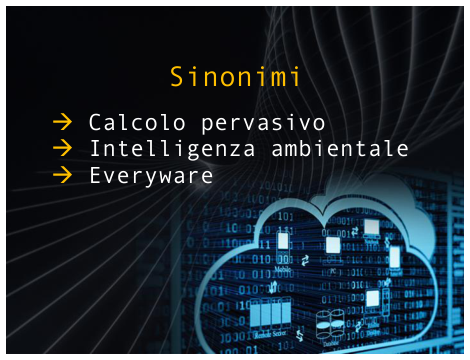
\includegraphics[width=0.50\textwidth,
                    trim=40 140 40 40, % L B R T
                    clip]
                    {images/Lez12_p02_fig_02}
  % \caption{Sommario}
  % \label{fig:Lez15_p06_fig_02}
\end{figure}
\FloatBarrier
\noindent

Ma vediamo alcuni sinonimi di calcolo ubiquo.
Calcolo ubiquo viene anche riferito come calcolo pervasivo che fa riferimento più all'indipendenza della localizzazione delle risorse ma il fatto che le risorse possano essere distribuite uniformemente o dovunque su un'area, su un territorio.

Intelligenza ambientale quindi pur offrendo un significato analogo focalizza l'attenzione sull'ambiente che comprende risorse di calcolo quindi intelligenza automatica.

Infine una nuova locuzione everyware con il suffisso analogo a hardware software logic or dataware a indicare l'insieme delle cose, l'insieme delle risorse di calcolo collocate ovunque.

\FloatBarrier
\begin{figure}[H]
  \centering
  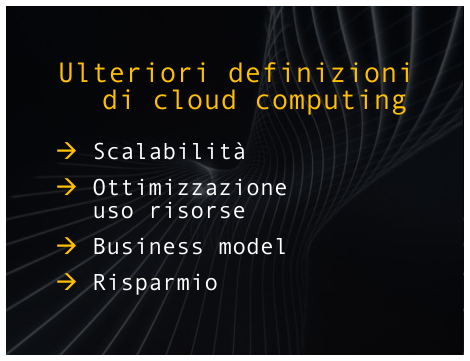
\includegraphics[width=0.50\textwidth,
                    trim=40 20 40 40, % L B R T
                    clip]
                    {images/Lez12_p02_fig_03}
  % \caption{Sommario}
  % \label{fig:Lez15_p06_fig_02}
\end{figure}
\FloatBarrier
\noindent

Vediamo ulteriori definizioni che vengono utilizzate per il cloud computing o meglio il focus che pongono.
Il primo è la scalabilità.
Definizioni di cloud computing che pur mantenendo caratteristiche essenziali di raggruppamento di risorse, erogazione di risorse a utenti esterni alla gestione del sistema, queste definizioni si riferiscono soprattutto alla scalabilità.

Scalabilità intende che le risorse disponibili sono molto più ampie della disponibilità di risorse fisiche grazie a meccanismi di virtualizzazione.

Altre definizioni focalizzano sull'ottimizzazione dell'uso delle risorse quindi il loro controllo, l'automazione della gestione e la riconfigurazione dinamica ed efficiente oppure il business model quindi il pagamento a uso e la collaborazione o l'economia, il risparmio perché con questo modello è possibile disporre di una quantità di risorse superiori alla quantità di risorse fisiche necessarie e non si deve acquistare la quantità di risorse fisiche che vengono erogate con questo servizio.

\FloatBarrier
\begin{figure}[H]
  \centering
  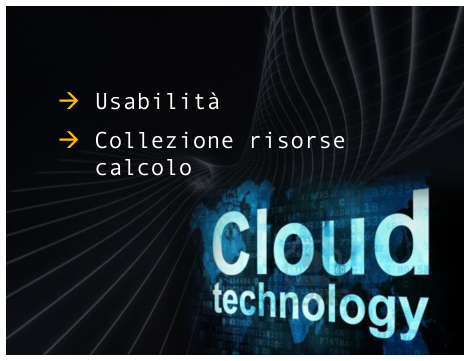
\includegraphics[width=0.50\textwidth,
                    trim=40 20 40 40, % L B R T
                    clip]
                    {images/Lez12_p02_fig_04}
  % \caption{Sommario}
  % \label{fig:Lez15_p06_fig_02}
\end{figure}
\FloatBarrier
\noindent

Altre definizioni focalizzano sull'usabilità quindi sulla disponibilità di interfacce, sulla facilità di richiesta di configurazione di questi servizi o d'altra parte sulla collezione delle risorse di calcolo quindi sul metodo che permette il raggruppamento e gestione di insiemi eterogenei di risorse che servono per una data applicazione per un dato servizio.

\section{Elemento cardine} %16:00

\FloatBarrier
\begin{figure}[H]
  \centering
  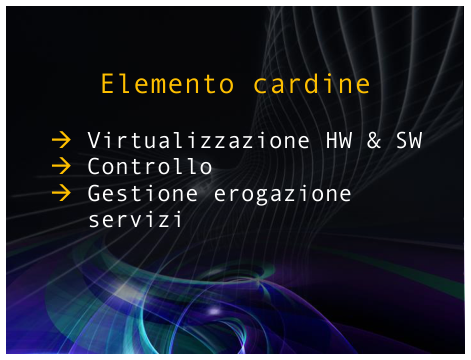
\includegraphics[width=0.50\textwidth,
                    trim=40 100 40 40, % L B R T
                    clip]
                    {images/Lez12_p02_fig_05}
  % \caption{Sommario}
  % \label{fig:Lez15_p06_fig_02}
\end{figure}
\FloatBarrier
\noindent



Un elemento cardine di questo modello è la virtualizzazione di hardware e di software che si intende che ogni risorsa viene presentata all'utente in forma simulata.

Uno degli elementi gestionali cardine di questo modello che presenta un sistema di calcolo, le risorse di calcolo, una rete, un sistema di archiviazione in forma virtuale potendone quindi estendere la disponibilità.

Un altro elemento è il controllo che richiede sia la misurazione delle risorse che sono erogate, la loro gestione completa, allocazione, rilascio e riassegnazione; l'erogazione corretta ed efficiente dei vari servizi.

\FloatBarrier
\begin{figure}[H]
  \centering
  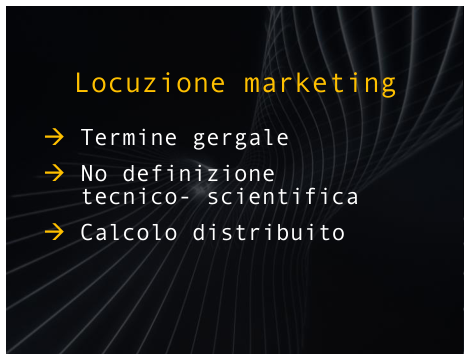
\includegraphics[width=0.50\textwidth,
                    trim=40 100 40 40, % L B R T
                    clip]
                    {images/Lez12_p02_fig_06}
  % \caption{Sommario}
  % \label{fig:Lez15_p06_fig_02}
\end{figure}
\FloatBarrier
\noindent


Il cloud computing è anche considerato una locuzione di marketing, un termine alla moda, un termine gergale e privo di una definizione tecnico scientifica che fa esclusivamente riferimento al calcolo distribuito.

\FloatBarrier
\begin{figure}[H]
  \centering
  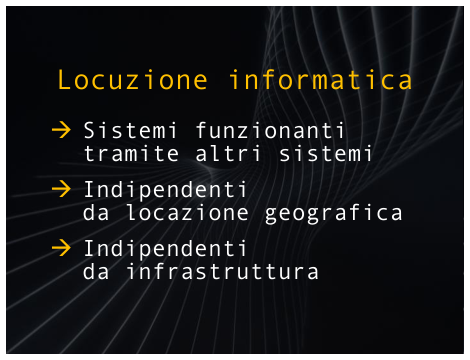
\includegraphics[width=0.50\textwidth,
                    trim=40 60 40 40, % L B R T
                    clip]
                    {images/Lez12_p03_fig_01}
  % \caption{Sommario}
  % \label{fig:Lez15_p06_fig_02}
\end{figure}
\FloatBarrier
\noindent

E' considerata una locazione informatica facente riferimento a sistemi funzionanti tramite altri sistemi; indipendenti dalla locazione geografica e indipendenti dalla infrastruttura di supporto.

\FloatBarrier
\begin{figure}[H]
  \centering
  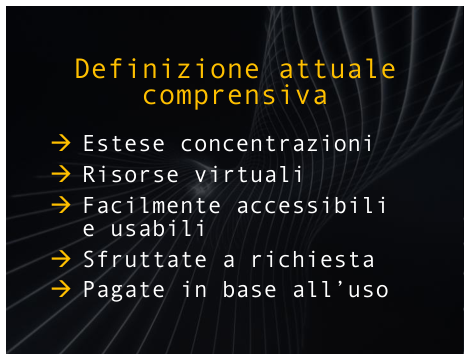
\includegraphics[width=0.50\textwidth,
                    trim=40 40 40 40, % L B R T
                    clip]
                    {images/Lez12_p03_fig_02}
  % \caption{Sommario}
  % \label{fig:Lez15_p06_fig_02}
\end{figure}
\FloatBarrier
\noindent

La definizione attuale e omnicomprensiva assimilata in ambito operativo considera il modello gestionale con estese concentrazioni di risorse che sono gestite in maniera virtuale, di fatto noi utenti, possiamo usufruire di una risorsa virtuale, di una simulazione dell'effettiva risorsa.

Le risorse sono facilmente accessibili e usabili, sono sfruttate a richiesta o da parte dell'utente o da parte del servizio attivato e, questa è una caratteristica fondante del modello, sono pagate a consumo.


Spunto di riflessione: confrontate il modello cloud che abbiamo appena presentato col modello per l'architettura client server dei servizi di rete.


\section{Modello di Cloud Computing}

\FloatBarrier
\begin{figure}[H]
  \centering
  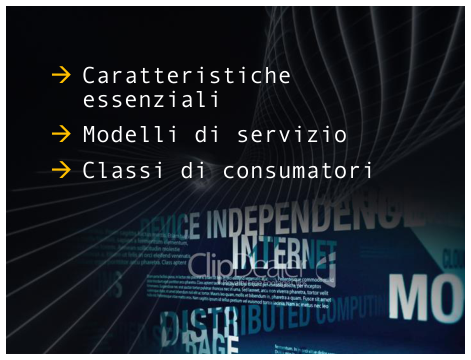
\includegraphics[width=0.50\textwidth,
                    trim=40 140 40 40, % L B R T
                    clip]
                    {images/Lez12_p03_fig_05}
  % \caption{Sommario}
  % \label{fig:Lez15_p06_fig_02}
\end{figure}
\FloatBarrier
\noindent

Il modello è costituito da tre elementi: le caratteristiche essenziali, i modelli di servizi che possono essere erogati e le classi di consumatori.

\subsection{Caratteristiche essenziali}%19:26

\FloatBarrier
\begin{figure}[H]
  \centering
  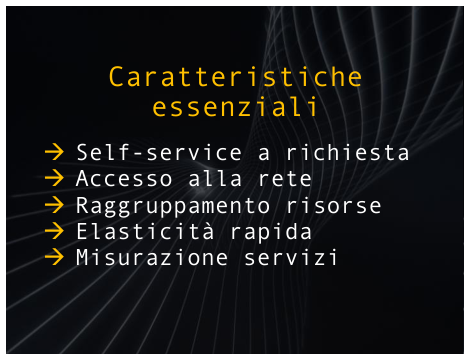
\includegraphics[width=0.50\textwidth,
                    trim=40 60 40 40, % L B R T
                    clip]
                    {images/Lez12_p03_fig_06}
  % \caption{Sommario}
  % \label{fig:Lez15_p06_fig_02}
\end{figure}
\FloatBarrier
\noindent

Le caratteristiche essenziali sono che il modello cloud computing è basato su risorse utilizzate autonomamente quindi self service e a richiesta.

L'accesso alla rete è basilare sia per accedere al servizio cloud che può essere remoto e delocalizzato, sia per permettere l'interazione tra cloud diversi; quindi la rete deve essere molto efficiente.

Il raggruppamento delle risorse necessarie all'erogazione complessiva di un servizio e la gestione veloce delle varie risorse, la gestione efficiente; l'overload, il sovraccarico di lavoro gestionale deve essere trascurabile rispetto alla computazione principale richiesta dal servizio.

I servizi per essere erogati a richiesta e a consumo devono poter essere misurati.

\subsection{Self service a richiesta}

Vediamo nel dettaglio queste caratteristiche singolarmente.

\FloatBarrier
\begin{figure}[H]
  \centering
  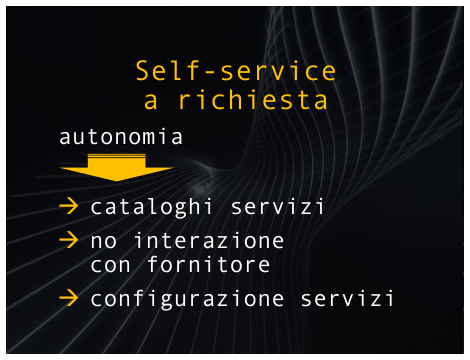
\includegraphics[width=0.50\textwidth,
                    trim=40 40 40 40, % L B R T
                    clip]
                    {images/Lez12_p04_fig_01}
  % \caption{Sommario}
  % \label{fig:Lez15_p06_fig_02}
\end{figure}
\FloatBarrier
\noindent

Self service a richiesta è l'autonomia dell'utente che utilizza cataloghi di servizi che gli presentano la gamma di risorse e di servizi disponibili, quindi memorie, collegamenti in rete e la possibilità di utilizzare ambienti di sviluppo o infrastrutture hardware virtualizzate, ambienti di sviluppo per sistemi di archiviazione, gestioni di dati o di documenti, sicurezza, quindi eventualmente configurarsi i propri firewall, i propri device di protezione.

Inoltre è richiesta una minima interazione con il fornitore.

L'autonomia vuole proprio indicare che l'utente di un servizio cloud deve potersi configurare autonomamente i propri servizi, scegliersi le proprie risorse minimizzando i rapporti che possano essere richiesti al fornitore o l'intervento della sua professionalità, della sua capacità.

La configurazione dei servizi dipende dal tipo di servizio che l'utente ha chiesto.

All'utente non è lasciato campo libero su qualsiasi tipo di configurazione per le risorse gestite in ambito cloud, ma a seconda dei servizi richiesti e a seconda del tipo di cliente, a che classe di utenti appartenga, potrà effettuare una certa attività di amministrazione, quindi configurarsi l'applicazione richiesta piuttosto che la piattaforma di sviluppo, piuttosto che il tipo di accesso alla rete, piuttosto che le risorse fisiche simulate e virtualizzate che sono richieste.

\subsection{Accesso alla rete}

\FloatBarrier
\begin{figure}[H]
  \centering
  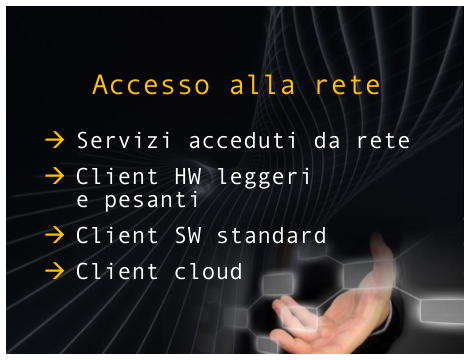
\includegraphics[width=0.50\textwidth,
                    trim=40 40 40 40, % L B R T
                    clip]
                    {images/Lez12_p04_fig_02}
  % \caption{Sommario}
  % \label{fig:Lez15_p06_fig_02}
\end{figure}
\FloatBarrier
\noindent

I servizi sono acceduti dalla rete, le risorse sono delocalizzate, tutte le risorse di calcolo sono disponibili indipendentemente dalla loro collocazione, sia geografica, sia nell'ambiente di calcolo, quindi dovranno conseguentemente essere acceduti dalla rete che dovrà essere efficiente anche perché l'obiettivo primario del modello cloud essendo il soddisfacimento di una richiesta di servizi da parte dell'utente è possibile che richieda accesso a un cloud supplementare, a un altro cloud, quindi accesso ai servizi del cloud e attraverso la rete e collegamento in rete anche di cloud differenti.

Client hardware leggeri e pesanti sono utilizzabili per la richiesta di servizi.

Abbiamo visto che i device, i client hardware da cui sono accessibili i servizi possono essere utilizzati in maniera interattiva da una persona ma possono essere anche utilizzati da applicazioni, quindi effettuare richieste automatiche.

Il client viene chiamato leggero quando effettua solo operazioni di richiesta, quindi nel servizio erogato la quantità di calcolo è limitata solitamente allo scambio per l'interazione, mentre i client pesanti possono erogare una maggiore quantità di calcolo per lo svolgimento di questo servizio.

I client software utilizzabili possono essere client standard quali browser di rete, applicativi per la posta o client che sono diventati standard de facto in ambito mobile, oppure anche client cloud, quindi client software specifici per l'uso semplificato e efficace del servizio e possono essere forniti ed eventualmente anche sviluppati dai fornitori stessi del servizio.

\subsection{Raggruppamento delle risorse} %27:04

\FloatBarrier
\begin{figure}[H]
  \centering
  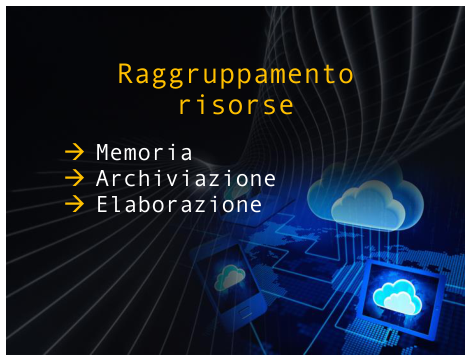
\includegraphics[width=0.50\textwidth,
                    trim=40 120 40 40, % L B R T
                    clip]
                    {images/Lez12_p04_fig_03}
  % \caption{Sommario}
  % \label{fig:Lez15_p06_fig_02}
\end{figure}
\FloatBarrier
\noindent

La memoria è una delle risorse di calcolo che possono essere erogate dai modelli cloud, insieme a sistemi di archiviazione della più ampia scelta possono essere offerti servizi di organizzazione di dati strutturati, di DMS, database management system, oppure sistemi di information retrieval per la gestione di dati narrativi o altri tipi di organizzazione, content management system, sistemi di gestione dei documenti o anche di immagini.

Inoltre sono collegate, raggruppate risorse per l'elaborazione quindi risorse di calcolo, calcolatori o sistemi più complessi, cluster di calcolatori, reti di calcolatori, insieme di calcolatori strutturati in qualsivoglia maniera che vengono gestiti da livello middleware e di virtualizzazione del cloud.

\FloatBarrier
\begin{figure}[H]
  \centering
  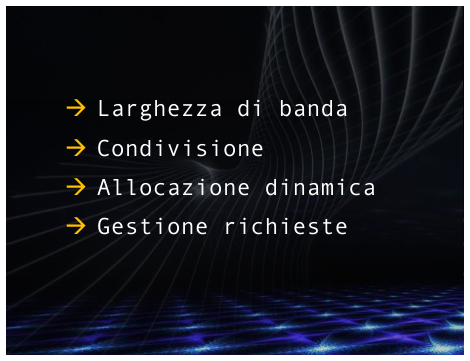
\includegraphics[width=0.50\textwidth,
                    trim=40 100 40 60, % L B R T
                    clip]
                    {images/Lez12_p04_fig_04}
  % \caption{Sommario}
  % \label{fig:Lez15_p06_fig_02}
\end{figure}
\FloatBarrier
\noindent

La larghezza di banda è basilare perché i servizi vengono erogati nella quasi totalità, non viene escluso l'accesso dall'organizzazione che ospita le risorse fisiche del cloud, ma il tipo di servizio è predisposto per l'accesso da remoto e quindi la larghezza di banda, la velocità di trasferimento dei dati è un fattore di basilare importanza per la qualità del servizio.

La condivisione delle risorse sia per l'utilizzo da parte delle varie altre risorse di calcolo che ne facessero richiesta, sia anche da parte direttamente degli utenti che avessero manifestato, effettuato una richiesta contemporanea di una risorsa di calcolo analoga o di una risorsa di memorizzazione o naturalmente dell'accesso alla rete.

L'allocazione dinamica delle risorse, quindi la misurazione, l'allocazione, il rilascio, l'assegnazione a un nuovo richiedente automatico o umano e la gestione complessiva delle richieste sono elementi fondamentali e devono essere efficaci ed efficienti per la gestione di raggruppamenti di risorse, di memoria, archiviazione, elaborazione e di collegamento, quindi per poter gestire effettivamente il pooling e il raggruppamento delle varie risorse di calcolo, erogando servizi di qualità.

\subsection{Elasticità rapida}

\FloatBarrier
\begin{figure}[H]
  \centering
  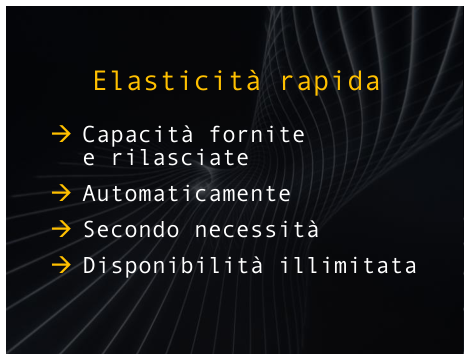
\includegraphics[width=0.50\textwidth,
                    trim=40 60 40 60, % L B R T
                    clip]
                    {images/Lez12_p04_fig_05}
  % \caption{Sommario}
  % \label{fig:Lez15_p06_fig_02}
\end{figure}
\FloatBarrier
\noindent

L'elasticità rapida è la capatià di fornire e rilasciare; la gestione del servizi a richiesta e a consumo richiede velocità, l'efficienza nel sapere quante risorse sono state utilizzate, quante ne serviranno e dove poter riperire in un dato estante una risorsa disponibile.

Vedremo che un livello dell'architettura logica del modello che implementa il modello cloud computing è un livello di middleware di gestione delle varie risorse e integrazione dei vari elementi di calcolo per fornire, erogare i servizi richiesti dagli utenti.

La gestione deve essere secondo le necessità per la richiesta e secondo le necessità del calcolo in atto; quindi se una computazione sta esaurendo una risorsa e si presume possa averne necessità nell'avanzamento del calcolo, ecco che il sistema di gestione deve mettere a disposizione la nuova risorsa necessaria per dare continuità alla computazione.

La disponibilità delle risorse è illimitata.
La virtualizzazione che è l'elemento fondamentale nel modello cloud computing permette, pur disponendo in un dato istante di una quantità finita di risorse di calcolo, di erogarne una quantità superiore, senza limiti.

Le risorse sono finite ma all'utente può essere mostrata una quantità di risorse senza limiti per soddisfare tutte le sue richieste o le necessità che venissero manifestate durante l'erogazione dei servizi dagli applicativi.

\subsection{Misurazione dei servizi} %33:32

\FloatBarrier
\begin{figure}[H]
  \centering
  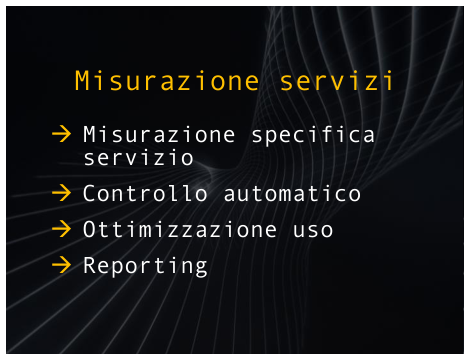
\includegraphics[width=0.50\textwidth,
                    trim=40 60 40 60, % L B R T
                    clip]
                    {images/Lez12_p04_fig_06}
  % \caption{Sommario}
  % \label{fig:Lez15_p06_fig_02}
\end{figure}
\FloatBarrier
\noindent

Misurazione specifica del servizio; per una gestione dinamica delle risorse ogni utilizzo di risorsa va misurato.

Il sistema deve sapere durante l'erogazione di un servizio quante risorse ha utilizzato, sta utilizzando, quante risorse possono essere necessarie per il calcolo immediato e successivo e dove sono reperibili eventuali risorse che si manifestassero necessarie; questo attraverso un controllo automatico.

Il calcolo necessario all'erogazione di un servizio deve essere sostenuto in maniera continua, offrendo all'erogazione del servizio una continuità per garantire la qualità del servizio stesso e ottimizzarne l'uso.

Il reporting, la produzione tabellare o di relazioni riguardanti l'uso delle risorse verrà prodotta per fornire al personale gestore del servizio i dati di misurazione effettuati sul servizio.

Vediamo alcune ulteriori caratteristiche. %35:42

\FloatBarrier
\begin{figure}[H]
  \centering
  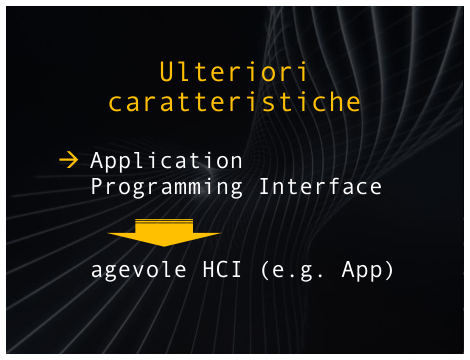
\includegraphics[width=0.50\textwidth,
                    trim=40 60 40 40, % L B R T
                    clip]
                    {images/Lez12_p05_fig_01}
  % \caption{Sommario}
  % \label{fig:Lez15_p06_fig_02}
\end{figure}
\FloatBarrier
\noindent

L'application programming interface, l'interfaccia di programmazione applicativa rende agevole la human computer interaction, quindi l'interazione uomo-machina, ad esempio per sviluppare delle app.

Per sostenere il distacco tra utente e fornitore vengono definite delle interfacce agevoli, delle interfacce usabili, facili e possibilmente interfacce, adesso chiamate app, per device mobili, device remoti, client leggeri.

\FloatBarrier
\begin{figure}[H]
  \centering
  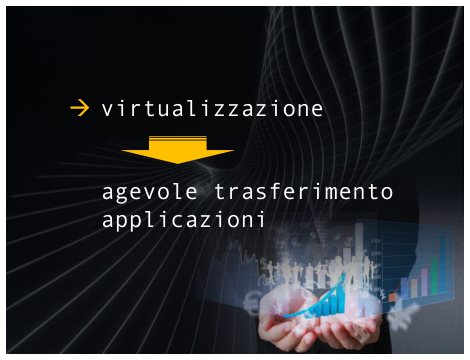
\includegraphics[width=0.50\textwidth,
                    trim=40 100 40 80, % L B R T
                    clip]
                    {images/Lez12_p05_fig_02}
  % \caption{Sommario}
  % \label{fig:Lez15_p06_fig_02}
\end{figure}
\FloatBarrier
\noindent

Inoltre abbiamo visto la virtualizzazione per l'agevole trasferimento delle applicazioni.

La virtualizzazione è uno degli elementi basilari per l'erogazione illimitata delle risorse per una gestione dinamica ma fornisce anche un vantaggio per il trasferimento di applicazioni che non sono dipendenti dalla risorsa fisica che gestiscono, che utilizzano.

\FloatBarrier
\begin{figure}[H]
  \centering
  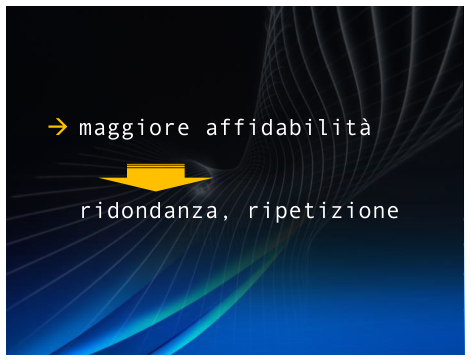
\includegraphics[width=0.50\textwidth,
                    trim=40 120 40 80, % L B R T
                    clip]
                    {images/Lez12_p05_fig_03}
  % \caption{Sommario}
  % \label{fig:Lez15_p06_fig_02}
\end{figure}
\FloatBarrier
\noindent
%%%%%%%%%%%%%%%%%%%%%%%%%%%%%%%%%%%%%38:10%%%%%%%%%%%%%%%%%%%%%%%%%%%%%%%%%%%%%%%%%


Una maggiore affidabilità proviene dalla ridondanza e dalla ripetizione delle risorse.

La virtualizzazione facilita la duplicazione sia delle risorse di calcolo, delle macchine virtuali, sia anche degli archivi memorizzati a scopo di backup o salvaguardia da eventuali guasti, interruzioni del servizio.

\FloatBarrier
\begin{figure}[H]
  \centering
  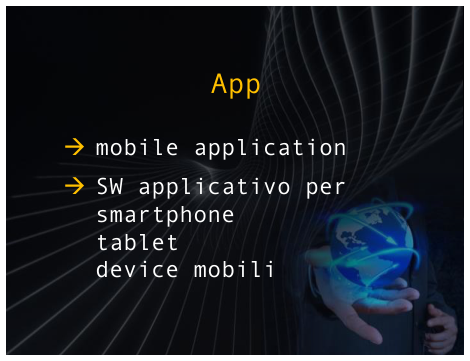
\includegraphics[width=0.50\textwidth,
                    trim=40 60 40 60, % L B R T
                    clip]
                    {images/Lez12_p05_fig_04}
  % \caption{Sommario}
  % \label{fig:Lez15_p06_fig_02}
\end{figure}
\FloatBarrier
\noindent

Le app sono applicazioni mobili, software applicativo che viene utilizzato per applicazioni su client leggeri, quali smartphone piuttosto che tablet, piuttosto che altri device mobili.

App è una locuzione che si è diffusa con questo tipo di applicazione nel 2008 e nel 2010 è stato considerato il termine dell'anno negli Stati Uniti.

\FloatBarrier
\begin{figure}[H]
  \centering
  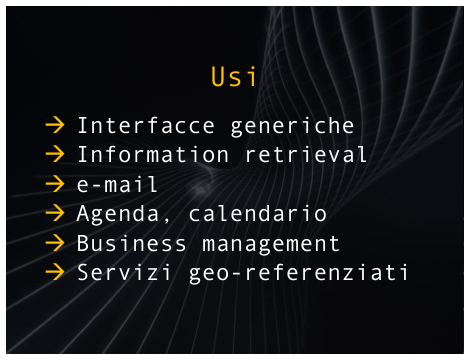
\includegraphics[width=0.50\textwidth,
                    trim=40 60 40 60, % L B R T
                    clip]
                    {images/Lez12_p05_fig_05}
  % \caption{Sommario}
  % \label{fig:Lez15_p06_fig_02}
\end{figure}
\FloatBarrier
\noindent

Queste app vengono utilizzati sia per interfacce generiche, soprattutto per richieste di informazioni, accesso ad archivi piuttosto che gestione di email o utilizzo di agende o calendari.

Inoltre è possibile l'uso di sistemi più complessi per la gestione di organizzazione, quindi business management piuttosto che accesso a sistemi informativi aziendali o servizi georeferenziati, geolocalizzati.

\FloatBarrier
\begin{figure}[H]
  \centering
  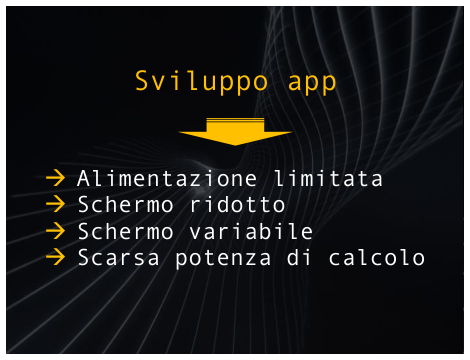
\includegraphics[width=0.50\textwidth,
                    trim=40 60 40 60, % L B R T
                    clip]
                    {images/Lez12_p05_fig_06}
  % \caption{Sommario}
  % \label{fig:Lez15_p06_fig_02}
\end{figure}
\FloatBarrier
\noindent

I limiti dello sviluppo delle applicazioni sono dovute ai device che li gestiscono, hanno un'alimentazione limitata, lo schermo solitamente è molto ridotto e variabile, nel senso che i device fisici sono di tipi molto differenti; offrono una scarsa potenza fisica di calcolo.

Spunto di riflessione: Nella vostra realtà lavorativa o formativa individuate quali servizi gestirete secondo il modello cloud, argomentate.